% answers.tex —— 2014 年·北京卷·理科 · 参考答案与详细解析片段
% 由 tools/generate_projects.py 依来源总账自 2014/2014_数学真题_北京理_试题.md + 2014/2014_数学真题_北京理_解析正文.md + 2014/2014_数学真题_北京理_答案要点.md 生成，勿手改（改源 MD 后重跑）


\begin{answer}
\gksolhead{1}{}

\textbf{题目}：

已知集合 $A=\{x\mid x^2-2x=0\}$，$B=\{0,1,2\}$，则 $A\cap B=$\mbox{（　　）}

（A）$\{0\}$；（B）$\{0,1\}$；（C）$\{0,2\}$；（D）$\{0,1,2\}$。

\Needspace{4\baselineskip}
\textbf{解析}

由 $x^2-2x=x(x-2)=0$ 得 $x=0$ 或 $x=2$，故 $A=\{0,2\}$。

\Needspace{5\baselineskip}
与 $B=\{0,1,2\}$ 取交集，共同元素为 $0$ 与 $2$，所以
\nopagebreak[4]
\[A\cap B=\{0,2\},\]
选 C。

\gkanswer{答案：C。$x^2-2x=0$ 给出 $x=0$ 或 $x=2$，故 $A=\{0,2\}$，$A\cap B=\{0,2\}$。}

\end{answer}
\begin{answer}
\gksolhead{2}{}

\textbf{题目}：

下列函数中，在区间 $(0,+\infty)$ 上为增函数的是\mbox{（　　）}

（A）$y=\sqrt{x+1}$；（B）$y=(x-1)^2$；（C）$y=2^{-x}$；（D）$y=\log_{0.5}(x+1)$。

\Needspace{4\baselineskip}
\textbf{解析}

逐个检查在 $(0,+\infty)$ 上的单调性：

\begin{itemize}
\item $y=\sqrt{x+1}$：定义域 $[-1,+\infty)$，$x$ 增大时 $x+1$ 增大，函数值随之增大，是增函数；
\item $y=(x-1)^2$：在 $(0,1)$ 上随 $x$ 增大而减小，不是增函数；
\item $y=2^{-x}$：底数 $2>1$，指数 $-x$ 递减，故函数递减；
\item $y=\log_{0.5}(x+1)$：底数 $0.5<1$，在 $(0,+\infty)$ 上递减。
\end{itemize}

只有第一项符合，选 A。

\gkanswer{答案：A。$y=\sqrt{x+1}$ 在 $(0,+\infty)$ 上递增；其余三项或递减，或在 $(0,1)$ 上递减。}

\end{answer}
\begin{answer}
\gksolhead{3}{}

\textbf{题目}：

\Needspace{5\baselineskip}
曲线
\nopagebreak[4]
\[\begin{cases}
x=-1+\cos\theta,\\
y=2+\sin\theta
\end{cases}\]
（$\theta$ 为参数）的对称中心\mbox{（　　）}

（A）在直线 $y=2x$ 上；（B）在直线 $y=-2x$ 上；（C）在直线 $y=x-1$ 上；（D）在直线 $y=x+1$ 上。

\Needspace{4\baselineskip}
\textbf{解析}

\Needspace{5\baselineskip}
由参数方程得 $x+1=\cos\theta$，$y-2=\sin\theta$，两式平方相加消去 $\theta$：
\nopagebreak[4]
\[(x+1)^2+(y-2)^2=1 .\]
曲线是圆心为 $(-1,2)$、半径为 $1$ 的圆，其对称中心即圆心 $(-1,2)$。

逐条代入检验：直线 $y=2x$ 给出 $2=-2$，不成立；直线 $y=-2x$ 给出 $2=2$，成立。故对称中心在直线 $y=-2x$ 上，选 B。

\gkanswer{答案：B。曲线是圆心为 $(-1,2)$、半径为 $1$ 的圆，圆心满足 $2=-2\times(-1)$，在直线 $y=-2x$ 上。}

\end{answer}
\begin{answer}
\gksolhead{4}{}

\textbf{题目}：

当 $m=7$，$n=3$ 时，执行如图所示的程序框图，输出的 $S$ 值为\mbox{（　　）}
\nopagebreak[4]
\begin{center}% ============================================================
% f2014_beijing_science_q04_flowchart.tex
% 2014 北京卷（理科）第 4 题：程序框图
% 来源 PDF：普通高考/2014/2014北京理.pdf
% 原页：第 1 页（A3），印面 861，左栏第 4 题题干下方
% 结构：开始 → 输入 m, n 的值 → k=m, S=1 → 判断 k<m-n+1；
%       否则 S=S·k、k=k-1 后返回判断；是则输出 S，再结束。
% ============================================================
\begin{tikzpicture}[>=Stealth, line width=0.7pt, font=\small]
  % 开始
  \draw[rounded corners=6pt] (-0.95,0.45) rectangle (0.95,-0.45);
  \node at (0,0) {开始};
  \draw[->] (0,-0.45) -- (0,-1.05);

  % 输入
  \draw (-2.00,-1.05) -- (1.70,-1.05) -- (2.00,-2.05) -- (-1.70,-2.05) -- cycle;
  \node at (0,-1.55) {输入 $m$，$n$ 的值};
  \draw[->] (0,-2.05) -- (0,-2.55);

  % 初始化
  \draw (-1.55,-2.55) rectangle (1.55,-3.45);
  \node at (0,-3.00) {$k=m$，$S=1$};
  \draw[->] (0,-3.45) -- (0,-4.33);

  % 判断菱形
  \draw (0,-4.35) -- (2.20,-5.35) -- (0,-6.35) -- (-2.20,-5.35) -- cycle;
  \node at (0,-5.35) {$k<m-n+1$};

  % 是：输出
  \draw[->] (0,-6.35) -- (0,-6.85);
  \node at (-0.40,-6.60) {是};
  \draw (-2.00,-6.85) -- (1.60,-6.85) -- (2.00,-7.85) -- (-1.60,-7.85) -- cycle;
  \node at (0,-7.35) {输出 $S$};
  \draw[->] (0,-7.85) -- (0,-8.35);

  % 结束
  \draw[rounded corners=6pt] (-0.95,-8.35) rectangle (0.95,-9.25);
  \node at (0,-8.80) {结束};

  % 否：循环体
  \draw[->] (2.20,-5.35) -- (2.90,-5.35);
  \node at (2.52,-5.08) {否};
  \draw (2.90,-5.85) rectangle (5.10,-4.85);
  \node at (4.00,-5.35) {$S=S\cdot k$};
  \draw[->] (4.00,-4.85) -- (4.00,-4.15);
  \draw (2.90,-4.15) rectangle (5.10,-3.15);
  \node at (4.00,-3.65) {$k=k-1$};

  % 回边：由 k=k-1 向左汇入判断框上方的竖线
  \draw[->] (2.90,-3.65) -- (0,-3.65);
\end{tikzpicture}
\end{center}
\nopagebreak[4]
（A）$7$；（B）$42$；（C）$210$；（D）$840$。

\Needspace{4\baselineskip}
\textbf{解析}

$m=7$，$n=3$ 时 $m-n+1=5$。初值 $k=7$，$S=1$。

判断 $k<5$ 不成立，执行循环体，再返回判断：

\begin{itemize}
\item $k=7$：$S=1\times7=7$，$k=6$；
\item $k=6$：$S=7\times6=42$，$k=5$；
\item $k=5$：$S=42\times5=210$，$k=4$；
\item $k=4<5$ 成立，输出 $S=210$。
\end{itemize}

即 $S=7\times6\times5=210$，选 C。

\gkanswer{答案：C。$m-n+1=5$，循环结束时 $S=7\times6\times5=210$。}

\end{answer}
\begin{answer}
\gksolhead{5}{}

\textbf{题目}：

设 $\{a_n\}$ 是公比为 $q$ 的等比数列，则“$q>1$”是“$\{a_n\}$ 为递增数列”的\mbox{（　　）}

（A）充分且不必要条件；（B）必要且不充分条件；（C）充分必要条件；（D）既不充分也不必要条件。

\Needspace{4\baselineskip}
\textbf{解析}

充分性：取 $a_1=-1$，$q=2>1$，则 $a_n=-2^{n-1}$，随 $n$ 增大而减小，不是递增数列，故“$q>1$”推不出递增。

必要性：取 $a_1=-1$，$q=\dfrac12<1$，则 $a_n=-2^{1-n}$，随 $n$ 增大而增大，是递增数列，故递增也推不出“$q>1$”。

因此是既不充分也不必要条件，选 D。

\gkanswer{答案：D。取 $a_1=-1$，$q=2$ 说明不充分；取 $a_1=-1$，$q=\dfrac12$ 说明不必要。}

\end{answer}
\begin{answer}
\gksolhead{6}{}

\textbf{题目}：

\Needspace{5\baselineskip}
若 $x$，$y$ 满足
\nopagebreak[4]
\[\begin{cases}
x+y-2\geqslant 0,\\
kx-y+2\geqslant 0,\\
y\geqslant 0,
\end{cases}\]
且 $z=y-x$ 的最小值为 $-4$，则 $k$ 的值为\mbox{（　　）}

（A）$2$；（B）$-2$；（C）$\dfrac12$；（D）$-\dfrac12$。

\Needspace{4\baselineskip}
\textbf{解析}

可行域为 $y\geqslant\max\{0,2-x\}$ 且 $y\leqslant kx+2$。

若 $k\geqslant0$，在 $y=0$ 上让 $x\to+\infty$ 仍满足全部条件，而 $z=y-x\to-\infty$，最小值不存在，故 $k<0$。

\Needspace{5\baselineskip}
若 $k<-1$：由 $y\geqslant2-x$ 与 $y\leqslant kx+2$ 得
\nopagebreak[4]
\[2-x\leqslant kx+2\iff x(1+k)\geqslant0 .\]
\Needspace{5\baselineskip}
而 $1+k<0$，故 $x\leqslant0$，此时 $y\geqslant2-x$，于是
\nopagebreak[4]
\[z=y-x\geqslant 2-2x\geqslant2,\]
最小值不为 $-4$，排除。

\Needspace{5\baselineskip}
若 $-1\leqslant k<0$：在 $y=0$ 上可行点满足 $2\leqslant x\leqslant-\dfrac2k$，且 $x<2$ 时 $z\geqslant2-2x>-2$。故最小值在 $y=0$、$x=-\dfrac2k$ 处取得：
\nopagebreak[4]
\[z_{\min}=-x=\frac2k .\]
\Needspace{5\baselineskip}
令 $\dfrac2k=-4$，得
\nopagebreak[4]
\[k=-\frac12,\]
它满足 $-1\leqslant k<0$。选 D。

\gkanswer{答案：D。$k<0$ 时由 $y=0$ 上 $2\leqslant x\leqslant-\dfrac2k$ 得 $z_{\min}=\dfrac2k$，令其为 $-4$ 得 $k=-\dfrac12$。}

\end{answer}
\begin{answer}
\gksolhead{7}{}

\textbf{题目}：

在空间直角坐标系 $Oxyz$ 中，已知 $A(2,0,0)$，$B(2,2,0)$，$C(0,2,0)$，$D(1,1,\sqrt2)$，若 $S_1$，$S_2$，$S_3$ 分别表示三棱锥 $D\text{-}ABC$ 在 $xOy$，$yOz$，$zOx$ 坐标平面上的正投影图形的面积，则\mbox{（　　）}

（A）$S_1=S_2=S_3$；（B）$S_1=S_2$ 且 $S_3\neq S_1$；（C）$S_1=S_3$ 且 $S_3\neq S_2$；（D）$S_2=S_3$ 且 $S_1\neq S_3$。

\Needspace{4\baselineskip}
\textbf{解析}

\Needspace{5\baselineskip}
三棱锥在 $xOy$ 平面上的投影：$D$ 的投影为 $D_1(1,1,0)$，它满足 $x+y=2$，落在边 $AC$ 上，故投影恰为 $\triangle ABC$，其中 $A(2,0)$，$B(2,2)$，$C(0,2)$，
\nopagebreak[4]
\[S_1=\frac12\cdot2\cdot2=2 .\]

\Needspace{5\baselineskip}
在 $yOz$ 平面上：$A$，$B$，$C$ 的投影分别为 $(0,0)$，$(2,0)$，$(2,0)$，$D$ 的投影为 $(1,\sqrt2)$，三点为 $(0,0)$，$(2,0)$，$(1,\sqrt2)$，
\nopagebreak[4]
\[S_2=\frac12\cdot2\cdot\sqrt2=\sqrt2 .\]

\Needspace{5\baselineskip}
在 $zOx$ 平面上：$A$，$B$，$C$ 的投影分别为 $(2,0)$，$(2,0)$，$(0,0)$，$D$ 的投影为 $(1,\sqrt2)$，
\nopagebreak[4]
\[S_3=\frac12\cdot2\cdot\sqrt2=\sqrt2 .\]

于是 $S_2=S_3=\sqrt2\neq2=S_1$，选 D。

\gkanswer{答案：D。$S_1=2$，$S_2=S_3=\sqrt2$，故 $S_2=S_3$ 且 $S_1\neq S_3$。}

\end{answer}
\begin{answer}
\gksolhead{8}{}

\textbf{题目}：

学生的语文、数学成绩均被评定为三个等级，依次为“优秀”“合格”“不合格”。若学生甲的语文、数学成绩都不低于学生乙，且其中至少有一门成绩高于乙，则称“学生甲比学生乙成绩好”。如果一组学生中不存在哪位学生比另一位学生成绩好，并且不存在语文成绩相同、数学成绩也相同的两位学生，则这一组学生最多有\mbox{（　　）}

（A）$2$ 人；（B）$3$ 人；（C）$4$ 人；（D）$5$ 人。

\Needspace{4\baselineskip}
\textbf{解析}

把每名学生的成绩记作二元组 $(\text{语文},\text{数学})$，等级取 $3$，$2$，$1$（优秀、合格、不合格）。“甲比乙成绩好”即甲的两个分量都不小于乙且至少一个严格大于，也就是二元组按分量顺序严格占优。

题设条件说明这组学生的二元组两两互不相同，且任意两人之间不存在占优关系，即构成偏序集 $\{1,2,3\}^2$ 中的一条反链。

同一语文等级下至多有一人：若两人语文同等级而数学不同，则数学高者占优，矛盾。语文只有 $3$ 个等级，故人数不超过 $3$。

另一方面，$(\text{优秀},\text{不合格})$，$(\text{合格},\text{合格})$，$(\text{不合格},\text{优秀})$ 三人两两不可比，满足条件。故最多 $3$ 人，选 B。

\gkanswer{答案：B。同一语文等级至多一人，故人数不超过 $3$，而（优秀，不合格）、（合格，合格）、（不合格，优秀）三人可达。}

\end{answer}
\begin{answer}
\gksolhead{9}{}

\textbf{题目}：

复数 $\left(\dfrac{1+\mathrm i}{1-\mathrm i}\right)^2=$\gkblank{}。

\Needspace{4\baselineskip}
\textbf{解析}

\Needspace{5\baselineskip}
先化简分数：
\nopagebreak[4]
\[\frac{1+\mathrm i}{1-\mathrm i}=\frac{(1+\mathrm i)^2}{(1-\mathrm i)(1+\mathrm i)}=\frac{1+2\mathrm i+\mathrm i^2}{1-\mathrm i^2}=\frac{2\mathrm i}{2}=\mathrm i .\]
\Needspace{5\baselineskip}
故
\nopagebreak[4]
\[\left(\frac{1+\mathrm i}{1-\mathrm i}\right)^2=\mathrm i^2=-1 .\]

\gkanswer{答案：$-1$。$\dfrac{1+\mathrm i}{1-\mathrm i}=\mathrm i$，平方得 $-1$。}

\end{answer}
\begin{answer}
\gksolhead{10}{}

\textbf{题目}：

已知向量 $\boldsymbol a$，$\boldsymbol b$ 满足 $|\boldsymbol a|=1$，$\boldsymbol b=(2,1)$，且 $\lambda\boldsymbol a+\boldsymbol b=\boldsymbol 0$（$\lambda\in\mathbf R$），则 $|\lambda|=$\gkblank{}。

\Needspace{4\baselineskip}
\textbf{解析}

\Needspace{5\baselineskip}
由 $\lambda\boldsymbol a+\boldsymbol b=\boldsymbol 0$ 得 $\lambda\boldsymbol a=-\boldsymbol b$，两边取模：
\nopagebreak[4]
\[|\lambda|\,|\boldsymbol a|=|\boldsymbol b|=\sqrt{2^2+1^2}=\sqrt5 .\]
又 $|\boldsymbol a|=1$，故 $|\lambda|=\sqrt5$。

\gkanswer{答案：$\sqrt5$。由 $\lambda\boldsymbol a=-\boldsymbol b$ 得 $|\lambda|=|\boldsymbol b|=\sqrt{2^2+1^2}=\sqrt5$。}

\end{answer}
\begin{answer}
\gksolhead{11}{}

\textbf{题目}：

设双曲线 $C$ 经过点 $(2,2)$，且与 $\dfrac{y^2}4-x^2=1$ 具有相同渐近线，则 $C$ 的方程为\gkblank{}；渐近线方程为\gkblank{}。

\Needspace{4\baselineskip}
\textbf{解析}

\Needspace{5\baselineskip}
与 $\dfrac{y^2}4-x^2=1$ 具有相同渐近线的双曲线可设为
\nopagebreak[4]
\[\frac{y^2}4-x^2=\lambda\quad(\lambda\neq0).\]
\Needspace{5\baselineskip}
代入点 $(2,2)$：
\nopagebreak[4]
\[\lambda=\frac{2^2}4-2^2=1-4=-3 .\]
\Needspace{5\baselineskip}
故 $C$ 的方程为 $\dfrac{y^2}4-x^2=-3$，即
\nopagebreak[4]
\[\frac{x^2}3-\frac{y^2}{12}=1 .\]
\Needspace{5\baselineskip}
渐近线由 $\dfrac{y^2}4-x^2=0$ 定出，即 $y^2=4x^2$，故渐近线方程为
\nopagebreak[4]
\[y=\pm2x .\]

\gkanswer{答案：$\dfrac{x^2}3-\dfrac{y^2}{12}=1$；$y=\pm2x$。设 $\dfrac{y^2}4-x^2=\lambda$，代入 $(2,2)$ 得 $\lambda=-3$。}

\end{answer}
\begin{answer}
\gksolhead{12}{}

\textbf{题目}：

若等差数列 $\{a_n\}$ 满足 $a_7+a_8+a_9>0$，$a_7+a_{10}<0$，则当 $n=$\gkblank{}时，$\{a_n\}$ 的前 $n$ 项和最大。

\Needspace{4\baselineskip}
\textbf{解析}

\Needspace{5\baselineskip}
由等差中项，
\nopagebreak[4]
\[a_7+a_8+a_9=3a_8>0\ \Rightarrow\ a_8>0,\]
\nopagebreak[4]
\[a_7+a_{10}=a_8+a_9<0\ \Rightarrow\ a_9<-a_8<0 .\]
\Needspace{5\baselineskip}
于是
\nopagebreak[4]
\[S_8-S_7=a_8>0,\qquad S_9-S_8=a_9<0 .\]
$S_n$ 先增后减，在 $n=8$ 处最大。

\gkanswer{答案：$8$。由条件得 $a_8>0$，$a_9<0$，故前 $8$ 项和最大。}

\end{answer}
\begin{answer}
\gksolhead{13}{}

\textbf{题目}：

把 $5$ 件不同产品摆成一排，若产品 $A$ 与产品 $B$ 相邻，且产品 $A$ 与产品 $C$ 不相邻，则不同的摆法有\gkblank{}种。

\Needspace{4\baselineskip}
\textbf{解析}

\Needspace{5\baselineskip}
把 $A$，$B$ 捆成一个整体：内部有 $AB$，$BA$ 两种顺序，与其余 $3$ 件共 $4$ 个对象排列，得
\nopagebreak[4]
\[2\times4!=48\ \text{\text{种}}.\]

\Needspace{5\baselineskip}
其中 $A$ 与 $C$ 也相邻的情形：三件连成一块且 $A$ 居中，即 $BAC$ 或 $CAB$ 两种，与其余 $2$ 件共 $3$ 个对象排列，得
\nopagebreak[4]
\[2\times3!=12\ \text{\text{种}}.\]

\Needspace{5\baselineskip}
所求摆法为
\nopagebreak[4]
\[48-12=36\ \text{\text{种}}.\]
（直接验证：$A$ 的位置分四类，$B$ 占相邻位后 $C$ 避开另一相邻位，合计 $1\times3+2\times2+2\times2+1\times3=36$。）

\gkanswer{答案：$36$。$A$，$B$ 相邻共 $2\times4!=48$ 种，其中 $A$ 也与 $C$ 相邻的有 $2\times3!=12$ 种，相减得 $36$。}

\end{answer}
\begin{answer}
\gksolhead{14}{}

\textbf{题目}：

设函数 $f(x)=A\sin(\omega x+\varphi)$（$A$，$\omega$，$\varphi$ 是常数，$A>0$，$\omega>0$）。若 $f(x)$ 在区间 $\left[\dfrac\pi6,\dfrac\pi2\right]$ 上具有单调性，且 $f\left(\dfrac\pi2\right)=f\left(\dfrac{2\pi}3\right)=-f\left(\dfrac\pi6\right)$，则 $f(x)$ 的最小正周期为\gkblank{}。

\Needspace{4\baselineskip}
\textbf{解析}

\Needspace{5\baselineskip}
设最小正周期为 $T$，则 $\omega=\dfrac{2\pi}T$。$f$ 在 $\left[\dfrac\pi6,\dfrac\pi2\right]$ 上单调，而该区间长度为 $\dfrac\pi3$，对应的相角跨度为 $\dfrac{\omega\pi}3$，故
\nopagebreak[4]
\[\frac{\omega\pi}3\leqslant\pi,\qquad \omega\leqslant3 .\]

\Needspace{5\baselineskip}
记
\nopagebreak[4]
\[u_1=\frac{\omega\pi}2+\varphi,\qquad u_2=\frac{2\omega\pi}3+\varphi,\qquad u_3=\frac{\omega\pi}6+\varphi,\]
则 $u_2-u_1=\dfrac{\omega\pi}6\in\left(0,\dfrac\pi2\right]$。

\Needspace{5\baselineskip}
由 $f\left(\dfrac\pi2\right)=f\left(\dfrac{2\pi}3\right)$，即 $\sin u_1=\sin u_2$。两角差在 $\left(0,\dfrac\pi2\right]$ 内，不可能是 $2\pi$ 的倍数，故只有
\nopagebreak[4]
\[u_1+u_2\equiv\pi\pmod{2\pi},\quad\text{\text{即}}\quad \frac{7\omega\pi}6+2\varphi\equiv\pi\pmod{2\pi}. \tag{1}\]

由 $f\left(\dfrac{2\pi}3\right)=-f\left(\dfrac\pi6\right)$，即 $\sin u_2=-\sin u_3=\sin(-u_3)$，有两种可能：

\begin{itemize}
\item $u_2\equiv-u_3\pmod{2\pi}$，即
\end{itemize}
\nopagebreak[4]
\[\frac{5\omega\pi}6+2\varphi\equiv0\pmod{2\pi};\tag{2}\]
\begin{itemize}
\item $u_2\equiv\pi+u_3\pmod{2\pi}$，即 $\dfrac{\omega\pi}2\equiv\pi\pmod{2\pi}$，故
\end{itemize}
\nopagebreak[4]
\[\omega=2+4k\ (k\in\mathbf Z).\tag{3}\]

若 (1) 与 (2) 同时成立，两式相减得 $\dfrac{\omega\pi}3\equiv\pi\pmod{2\pi}$，即 $\omega=3+6k$，结合 $\omega\leqslant3$ 得 $\omega=3$。此时由 (2) 得 $\varphi\equiv-\dfrac\pi4\pmod\pi$：

\begin{itemize}
\item $\varphi=-\dfrac\pi4$ 时，$x\in\left[\dfrac\pi6,\dfrac\pi2\right]$ 对应 $u\in\left[\dfrac\pi4,\dfrac{5\pi}4\right]$，$\sin u$ 先增后减，不单调；
\item $\varphi=\dfrac{3\pi}4$ 时，$u\in\left[\dfrac{5\pi}4,\dfrac{9\pi}4\right]$，$\sin u$ 先减后增，也不单调。
\end{itemize}

故 $\omega\neq3$。

\Needspace{5\baselineskip}
若 (1) 与 (3) 同时成立，由 $\omega\leqslant3$ 且 $\omega>0$ 得 $\omega=2$，$T=\pi$。此时由 (1) 得
\nopagebreak[4]
\[\frac{7\pi}3+2\varphi\equiv\pi\pmod{2\pi},\qquad \varphi\equiv-\frac{2\pi}3\pmod\pi .\]
取 $\varphi=\dfrac\pi3$，则 $u=2x+\dfrac\pi3$ 在 $\left[\dfrac\pi6,\dfrac\pi2\right]$ 上从 $\dfrac{2\pi}3$ 增到 $\dfrac{4\pi}3$，$\sin u$ 在此区间上严格递减，单调性满足；取 $\varphi=-\dfrac{2\pi}3$ 时 $u$ 从 $-\dfrac\pi3$ 增到 $\dfrac\pi3$，严格递增，同样满足。

所以最小正周期为 $\pi$。

\gkanswer{答案：$\pi$。由相角条件只能取 $\omega=2$（$\omega=3$ 在题给区间上不单调）。}

\end{answer}
\begin{answer}
\gksolhead{15}{}

\textbf{题目}：

如图，在 $\triangle ABC$ 中，$\angle B=\dfrac\pi3$，$AB=8$，点 $D$ 在 $BC$ 上，且 $CD=2$，$\cos\angle ADC=\dfrac17$。
\nopagebreak[4]
\begin{center}% ============================================================
% f2014_beijing_science_q15_triangle.tex
% 2014 北京卷（理科）第 15 题：三角形 ABC 与点 D
% 来源 PDF：普通高考/2014/2014北京理.pdf
% 原页：第 1 页（A3），印面 861，中栏第 15 题题干下方
% 已知 ∠B=π/3，AB=8，CD=2；图按 AB=8、BD=3、DC=2、AC=7 的真实比例绘制。
% ============================================================
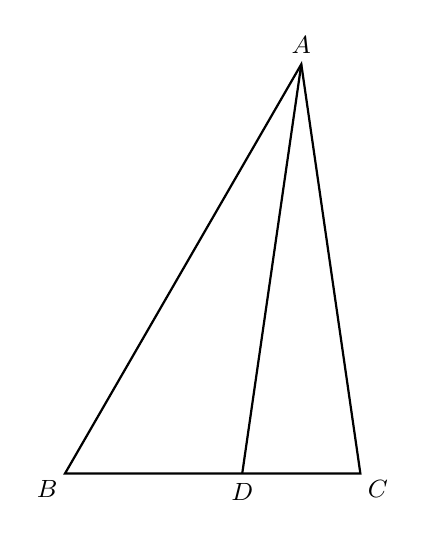
\begin{tikzpicture}[scale=0.75, line width=0.8pt, font=\small]
  \coordinate (B) at (0,0);
  \coordinate (D) at (3,0);
  \coordinate (C) at (5,0);
  \coordinate (A) at (4,6.9282);   % AB=8，∠B=60°

  \draw (A) -- (B) -- (C) -- cycle;
  \draw (A) -- (D);

  \node[above] at (A) {$A$};
  \node[below left=-1pt] at (B) {$B$};
  \node[below] at (D) {$D$};
  \node[below right=-1pt] at (C) {$C$};
\end{tikzpicture}
\end{center}
\nopagebreak[4]
（1） 求 $\sin\angle BAD$；

（2） 求 $BD$，$AC$ 的长。

\Needspace{4\baselineskip}
\textbf{解析}

\gksubpart{（1）}

\Needspace{5\baselineskip}
$\angle ADC$ 是 $\triangle ABD$ 在顶点 $D$ 处的外角，故
\nopagebreak[4]
\[\angle ADC=\angle ABD+\angle BAD=\frac\pi3+\angle BAD .\]
\Needspace{5\baselineskip}
由 $\cos\angle ADC=\dfrac17$ 且 $\angle ADC$ 为三角形内角，得
\nopagebreak[4]
\[\sin\angle ADC=\sqrt{1-\frac1{49}}=\frac{4\sqrt3}7 .\]
\Needspace{5\baselineskip}
于是
\nopagebreak[4]
\[\begin{aligned}
\sin\angle BAD&=\sin\left(\angle ADC-\frac\pi3\right)\\
&=\sin\angle ADC\cos\frac\pi3-\cos\angle ADC\sin\frac\pi3\\
&=\frac{4\sqrt3}7\cdot\frac12-\frac17\cdot\frac{\sqrt3}2\\
&=\frac{4\sqrt3-\sqrt3}{14}=\frac{3\sqrt3}{14}.
\end{aligned}\]

\gksubpart{（2）}

\Needspace{5\baselineskip}
在 $\triangle ABD$ 中，$\angle ADB=\pi-\angle ADC$，故 $\sin\angle ADB=\sin\angle ADC=\dfrac{4\sqrt3}7$。由正弦定理，
\nopagebreak[4]
\[\frac{BD}{\sin\angle BAD}=\frac{AB}{\sin\angle ADB},\]
\nopagebreak[4]
\[BD=8\cdot\frac{3\sqrt3/14}{4\sqrt3/7}=8\cdot\frac{3}{8}=3 .\]
故 $BC=BD+DC=3+2=5$。

\Needspace{5\baselineskip}
在 $\triangle ABC$ 中用余弦定理，
\nopagebreak[4]
\[AC^2=AB^2+BC^2-2\cdot AB\cdot BC\cos\frac\pi3=64+25-2\cdot8\cdot5\cdot\frac12=49,\]
所以 $AC=7$。

检验：$AD=7$（正弦定理），而 $\cos\angle ADC=\dfrac{AD^2+DC^2-AC^2}{2\cdot AD\cdot DC}=\dfrac{49+4-49}{28}=\dfrac17$，与题设一致。

\gkanswer{答案（1）：$\dfrac{3\sqrt3}{14}$。$\angle ADC=\dfrac\pi3+\angle BAD$，用两角差的正弦展开。}

\gkanswer{答案（2）：$BD=3$，$AC=7$。正弦定理得 $BD=3$，再由余弦定理得 $AC^2=49$。}

\end{answer}
\begin{answer}
\gksolhead{16}{}

\textbf{题目}：

李明在 $10$ 场篮球比赛中的投篮情况（假设各场比赛相互独立）：

\begin{center}
\begin{tabular}{llllll}
\toprule
场次 & 投篮次数 & 命中次数 & 场次 & 投篮次数 & 命中次数 \\
\midrule
主场 $1$ & $22$ & $12$ & 客场 $1$ & $18$ & $8$ \\
主场 $2$ & $15$ & $12$ & 客场 $2$ & $13$ & $12$ \\
主场 $3$ & $12$ & $8$ & 客场 $3$ & $21$ & $7$ \\
主场 $4$ & $23$ & $8$ & 客场 $4$ & $18$ & $15$ \\
主场 $5$ & $24$ & $20$ & 客场 $5$ & $25$ & $12$ \\
\bottomrule
\end{tabular}
\end{center}

（1） 从上述比赛随机选择一场，求李明在该场比赛中的投篮命中率超过 $0.6$ 的概率；

（2） 从上述比赛随机选择一个主场和客场，求李明的投篮命中率一场超过 $0.6$，一场不超过 $0.6$ 的概率；

（3） 记 $\bar x$ 是表中 $10$ 个命中次数的平均数，从上述比赛中随机选择一场，记 $X$ 为李明在这场比赛中命中次数，比较 $E(X)$ 与 $\bar x$ 的大小。（只需写出结论）

\Needspace{4\baselineskip}
\textbf{解析}

\gksubpart{（1）}

逐场计算命中率（命中次数除以投篮次数）：主场依次为 $\dfrac{12}{22}\approx0.545$，$\dfrac{12}{15}=0.8$，$\dfrac{8}{12}\approx0.667$，$\dfrac{8}{23}\approx0.348$，$\dfrac{20}{24}\approx0.833$；客场依次为 $\dfrac{8}{18}\approx0.444$，$\dfrac{12}{13}\approx0.923$，$\dfrac{7}{21}\approx0.333$，$\dfrac{15}{18}\approx0.833$，$\dfrac{12}{25}=0.48$。

\Needspace{5\baselineskip}
超过 $0.6$ 的共 $5$ 场（主场 $2$、$3$、$5$ 与客场 $2$、$4$），故所求概率为
\nopagebreak[4]
\[\frac5{10}=\frac12 .\]

\gksubpart{（2）}

随机选一个主场和一个客场，共有 $5\times5=25$ 个等可能的基本事件。

\Needspace{5\baselineskip}
主场中超过 $0.6$ 的有 $3$ 场、不超过的有 $2$ 场；客场中超过 $0.6$ 的有 $2$ 场、不超过的有 $3$ 场。恰有一场超过的配对数为
\nopagebreak[4]
\[3\times3+2\times2=9+4=13,\]
故所求概率为 $\dfrac{13}{25}$。

\gksubpart{（3）}

\Needspace{5\baselineskip}
$10$ 个命中次数之和为
\nopagebreak[4]
\[12+12+8+8+20+8+12+7+15+12=114,\]
故 $\bar x=\dfrac{114}{10}=11.4$。

\Needspace{5\baselineskip}
每场比赛被选中的概率都是 $\dfrac1{10}$，此时 $X$ 就取该场的命中次数，故
\nopagebreak[4]
\[E(X)=\frac1{10}\sum_{i=1}^{10}x_i=\bar x=11.4 .\]
两者相等。

\gkanswer{答案（1）：$\dfrac12$。$10$ 场中命中率超过 $0.6$ 的有 $5$ 场。}

\gkanswer{答案（2）：$\dfrac{13}{25}$。主场中 $3$ 场、客场中 $2$ 场超过 $0.6$，恰一场超过的配对数 $3\times3+2\times2=13$。}

\gkanswer{答案（3）：$E(X)=\bar x$。各场等可能，故 $E(X)$ 就是 $10$ 个命中次数的平均数 $11.4$。}

\end{answer}
\begin{answer}
\gksolhead{17}{}

\textbf{题目}：

如图，正方形 $AMDE$ 的边长为 $2$，$B$，$C$ 分别为 $AM$，$MD$ 的中点，在五棱锥 $P\text{-}ABCDE$ 中，$F$ 为棱 $PE$ 的中点，平面 $ABF$ 与棱 $PD$，$PC$ 分别交于点 $G$，$H$。
\nopagebreak[4]
\begin{center}% ============================================================
% f2014_beijing_science_q17_pyramid.tex
% 2014 北京卷（理科）第 17 题：五棱锥 P-ABCDE
% 来源 PDF：普通高考/2014/2014北京理.pdf
% 原页：第 1 页（A3），印面 861，右栏第 17 题题干下方
% 底面为正方形 AMDE（边长 2）截去 △MBC，B、C 分别为 AM、MD 中点；
% F 为 PE 中点，截面 ABF 与 PD、PC 交于 G、H，截面为五边形 ABHGF。
% 斜二测投影：px = X + 0.52Y，py = Z + 0.62Y（再乘 1.6 作尺寸）。
% ============================================================
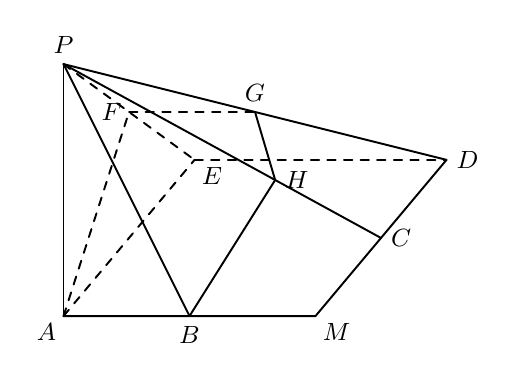
\begin{tikzpicture}[line width=0.7pt, font=\small,
  line cap=round, line join=round]
  % 顶点（斜二测投影后的纸面坐标）
  \coordinate (P)  at (0,3.200);
  \coordinate (A)  at (0,0);
  \coordinate (B)  at (1.600,0);
  \coordinate (M)  at (3.200,0);
  \coordinate (C)  at (4.032,0.992);
  \coordinate (D)  at (4.864,1.984);
  \coordinate (E)  at (1.664,1.984);
  \coordinate (F)  at (0.832,2.592);  % PE 中点
  \coordinate (G)  at (2.432,2.592);  % PD 中点
  \coordinate (H)  at (2.688,1.728);  % PC 上，PH:HC=2:1

  % 被遮挡的棱与截面边
  \draw[dashed] (P) -- (E);
  \draw[dashed] (A) -- (E);
  \draw[dashed] (E) -- (D);
  \draw[dashed] (A) -- (F);
  \draw[dashed] (F) -- (G);

  % 可见的棱
  \draw (P) -- (A);
  \draw (P) -- (B);
  \draw (P) -- (C);
  \draw (P) -- (D);
  \draw (A) -- (B) -- (M) -- (C) -- (D);

  % 可见的截面边
  \draw (B) -- (H) -- (G);

  % 标注
  \node[above] at (P) {$P$};
  \node[left=-1pt] at (F) {$F$};
  \node[above] at (G) {$G$};
  \node[right] at (H) {$H$};
  \node[below right=-1pt] at (E) {$E$};
  \node[below left=-1pt] at (A) {$A$};
  \node[below] at (B) {$B$};
  \node[below right=-1pt] at (M) {$M$};
  \node[right] at (C) {$C$};
  \node[right] at (D) {$D$};
\end{tikzpicture}
\end{center}
\nopagebreak[4]
（1） 求证：$AB\parallel FG$；

（2） 若 $PA\perp$ 平面 $ABCDE$，且 $PA=AE$，求直线 $BC$ 与平面 $ABF$ 所成角的大小，并求线段 $PH$ 的长。

\Needspace{4\baselineskip}
\textbf{解析}

\gksubpart{（1）}

\Needspace{5\baselineskip}
正方形 $AMDE$ 中 $AM\parallel DE$，而 $A$，$B$ 都在边 $AM$ 上，故
\nopagebreak[4]
\[AB\parallel DE .\]
$DE\subset$ 平面 $PDE$，$AB\not\subset$ 平面 $PDE$，故 $AB\parallel$ 平面 $PDE$。

\Needspace{5\baselineskip}
又 $F$ 在 $PE$ 上、$G$ 在 $PD$ 上，故 $F$，$G$ 都在平面 $PDE$ 内；同时 $F$，$G$ 都在平面 $ABF$ 内。于是
\nopagebreak[4]
\[\text{\text{平面} }ABF\cap\text{\text{平面} }PDE=FG .\]
由线面平行的性质定理，$AB\parallel FG$。

\gksubpart{（2）}

\Needspace{5\baselineskip}
以 $A$ 为原点，$\overrightarrow{AM}$ 为 $x$ 轴正方向，$\overrightarrow{AE}$ 为 $y$ 轴正方向，$\overrightarrow{AP}$ 为 $z$ 轴正方向建系。由 $AM=AE=2$，$B$，$C$ 为中点，$PA=AE=2$ 得
\nopagebreak[4]
\[A(0,0,0),\ B(1,0,0),\ C(2,1,0),\ D(2,2,0),\ E(0,2,0),\ P(0,0,2).\]
$F$ 为 $PE$ 中点，故 $F(0,1,1)$。

\Needspace{5\baselineskip}
$\overrightarrow{AB}=(1,0,0)$，$\overrightarrow{AF}=(0,1,1)$，取平面 $ABF$ 的法向量
\nopagebreak[4]
\[\boldsymbol n=(0,-1,1),\]
它满足 $\boldsymbol n\cdot\overrightarrow{AB}=0$，$\boldsymbol n\cdot\overrightarrow{AF}=0$。

\Needspace{5\baselineskip}
又 $\overrightarrow{BC}=(1,1,0)$。设直线 $BC$ 与平面 $ABF$ 所成角为 $\theta$，则
\nopagebreak[4]
\[\sin\theta=\frac{|\overrightarrow{BC}\cdot\boldsymbol n|}{|\overrightarrow{BC}|\,|\boldsymbol n|}=\frac{|-1|}{\sqrt2\cdot\sqrt2}=\frac12,\]
故 $\theta=\dfrac\pi6$。

\Needspace{5\baselineskip}
再求 $PH$。设 $H$ 分 $PC$ 的比为 $t$，即 $\overrightarrow{PH}=t\overrightarrow{PC}$（$0\leqslant t\leqslant1$）。由 $P(0,0,2)$，$C(2,1,0)$ 得
\nopagebreak[4]
\[H(2t,\,t,\,2-2t).\]
\Needspace{5\baselineskip}
平面 $ABF$ 的方程为 $-y+z=0$，代入得
\nopagebreak[4]
\[-t+(2-2t)=0\ \Rightarrow\ t=\frac23 .\]
\Needspace{5\baselineskip}
又
\nopagebreak[4]
\[|PC|=\sqrt{2^2+1^2+(-2)^2}=3,\]
\Needspace{5\baselineskip}
故
\nopagebreak[4]
\[PH=\frac23\,|PC|=2 .\]

\gkanswer{答案（1）：见解析版}

\gkanswer{答案（2）：所成角为 $\dfrac\pi6$，$PH=2$。以 $A$ 为原点建系，平面 $ABF$ 的法向量为 $(0,-1,1)$，$BC=(1,1,0)$，由 $\sin\theta=\dfrac12$ 得 $\theta=\dfrac\pi6$；$H$ 分 $PC$ 为 $2:1$，故 $PH=\dfrac23|PC|=2$。}

\end{answer}
\begin{answer}
\gksolhead{18}{}

\textbf{题目}：

已知函数 $f(x)=x\cos x-\sin x$，$x\in\left[0,\dfrac\pi2\right]$。

（1） 求证：$f(x)\leqslant 0$；

（2） 若 $a<\dfrac{\sin x}x<b$ 在 $\left(0,\dfrac\pi2\right)$ 上恒成立，求 $a$ 的最大值与 $b$ 的最小值。

\Needspace{4\baselineskip}
\textbf{解析}

\gksubpart{（1）}

\Needspace{5\baselineskip}
求导：
\nopagebreak[4]
\[f'(x)=\cos x-x\sin x-\cos x=-x\sin x .\]
当 $x\in\left(0,\dfrac\pi2\right)$ 时 $x>0$，$\sin x>0$，故 $f'(x)<0$，$f$ 在 $\left[0,\dfrac\pi2\right]$ 上严格递减。

\Needspace{5\baselineskip}
又 $f(0)=0\cdot1-0=0$，故对一切 $x\in\left[0,\dfrac\pi2\right]$ 有
\nopagebreak[4]
\[f(x)\leqslant f(0)=0 .\]

\gksubpart{（2）}

\Needspace{5\baselineskip}
令 $g(x)=\dfrac{\sin x}x$，$x\in\left(0,\dfrac\pi2\right)$。由商的求导法则，
\nopagebreak[4]
\[g'(x)=\frac{x\cos x-\sin x}{x^2}=\frac{f(x)}{x^2}\leqslant0,\]
\Needspace{5\baselineskip}
且 $x\in\left(0,\dfrac\pi2\right)$ 时 $f(x)<0$，故 $g$ 在 $\left(0,\dfrac\pi2\right)$ 上严格递减。于是
\nopagebreak[4]
\[\lim_{x\to0^+}g(x)=1,\qquad g\left(\frac\pi2\right)=\frac{\sin(\pi/2)}{\pi/2}=\frac2\pi,\]
$g$ 的值域为 $\left(\dfrac2\pi,1\right)$（两端点均取不到）。

\Needspace{5\baselineskip}
要使 $a<g(x)<b$ 在 $\left(0,\dfrac\pi2\right)$ 上恒成立，必须且只须
\nopagebreak[4]
\[a\leqslant\frac2\pi,\qquad b\geqslant1 .\]
故 $a$ 的最大值为 $\dfrac2\pi$，$b$ 的最小值为 $1$。

\gkanswer{答案（1）：见解析版}

\gkanswer{答案（2）：$a$ 的最大值为 $\dfrac2\pi$，$b$ 的最小值为 $1$。$\dfrac{\sin x}x$ 在 $\left(0,\dfrac\pi2\right)$ 上递减，值域为 $\left(\dfrac2\pi,1\right)$。}

\end{answer}
\begin{answer}
\gksolhead{19}{}

\textbf{题目}：

已知椭圆 $C:x^2+2y^2=4$。

（1） 求椭圆 $C$ 的离心率；

（2） 设 $O$ 为坐标原点，若点 $A$ 在椭圆 $C$ 上，点 $B$ 在直线 $y=2$ 上，且 $OA\perp OB$，试判断直线 $AB$ 与圆 $x^2+y^2=2$ 的位置关系，并证明你的结论。

\Needspace{4\baselineskip}
\textbf{解析}

\gksubpart{（1）}

\Needspace{5\baselineskip}
把方程写成标准形
\nopagebreak[4]
\[\frac{x^2}4+\frac{y^2}2=1,\]
\Needspace{5\baselineskip}
故 $a^2=4$，$b^2=2$，$c^2=a^2-b^2=2$，于是
\nopagebreak[4]
\[e=\frac ca=\frac{\sqrt2}{2} .\]

\gksubpart{（2）}

设 $A(2\cos\theta,\sqrt2\sin\theta)$，$B(t,2)$，其中 $\theta\in[0,2\pi)$。若 $\cos\theta=0$，则 $A=(0,\pm\sqrt2)$，由 $OA\perp OB$ 得 $\overrightarrow{OA}\cdot\overrightarrow{OB}=2\cdot(\pm\sqrt2)\neq0$，矛盾，故 $\cos\theta\neq0$。

\Needspace{5\baselineskip}
由 $OA\perp OB$：
\nopagebreak[4]
\[\overrightarrow{OA}\cdot\overrightarrow{OB}=2t\cos\theta+2\sqrt2\sin\theta=0\ \Rightarrow\ t=-\frac{\sqrt2\sin\theta}{\cos\theta} .\]

\Needspace{5\baselineskip}
原点到直线 $AB$ 的距离为
\nopagebreak[4]
\[d=\frac{|x_Ay_B-y_Ax_B|}{\sqrt{(x_A-t)^2+(y_A-2)^2}}
=\frac{\left|4\cos\theta+\dfrac{2\sin^2\theta}{\cos\theta}\right|}{|AB|}
=\frac{2(1+\cos^2\theta)}{|\cos\theta|\,|AB|} .\]

\Needspace{5\baselineskip}
又
\nopagebreak[4]
\[\begin{aligned}
|AB|^2&=\left(2\cos\theta+\frac{\sqrt2\sin\theta}{\cos\theta}\right)^2+\left(\sqrt2\sin\theta-2\right)^2\\
&=4\cos^2\theta+4\sqrt2\sin\theta+\frac{2\sin^2\theta}{\cos^2\theta}
+2\sin^2\theta-4\sqrt2\sin\theta+4\\
&=4\cos^2\theta+2\sin^2\theta+4+\frac{2\sin^2\theta}{\cos^2\theta}.
\end{aligned}\]
\Needspace{5\baselineskip}
记 $q=\cos^2\theta$，则 $\sin^2\theta=1-q$，于是
\nopagebreak[4]
\[|AB|^2=4q+2(1-q)+4+\frac{2(1-q)}q=2q+6+\frac{2(1-q)}q=\frac{2(q+1)^2}{q} .\]
\Needspace{5\baselineskip}
代入距离公式：
\nopagebreak[4]
\[d^2=\frac{4(1+q)^2}{q}\cdot\frac{q}{2(q+1)^2}=2,\]
故 $d=\sqrt2$。

圆 $x^2+y^2=2$ 的半径为 $\sqrt2$，而原点到直线 $AB$ 的距离恒等于 $\sqrt2$，所以直线 $AB$ 与该圆相切。

\gkanswer{答案（1）：$\dfrac{\sqrt2}2$。$a=2$，$b=\sqrt2$，$c=\sqrt2$。}

\gkanswer{答案（2）：直线 $AB$ 与圆 $x^2+y^2=2$ 相切。原点到 $AB$ 的距离恒为 $\sqrt2$，等于圆的半径。}

\end{answer}
\begin{answer}
\gksolhead{20}{}

\textbf{题目}：

对于数对序列 $P:(a_1,b_1),(a_2,b_2),\cdots,(a_n,b_n)$，记 $T_1(P)=a_1+b_1$，$T_k(P)=b_k+\max\{T_{k-1}(P),a_1+a_2+\cdots+a_k\}$（$2\leqslant k\leqslant n$），其中 $\max\{T_{k-1}(P),a_1+a_2+\cdots+a_k\}$ 表示 $T_{k-1}(P)$ 和 $a_1+a_2+\cdots+a_k$ 两个数中最大的数。

（1） 对于数对序列 $P:(2,5),(4,1)$，求 $T_1(P)$，$T_2(P)$ 的值；

（2） 记 $m$ 为 $a$，$b$，$c$，$d$ 四个数中最小值，对于由两个数对 $(a,b)$，$(c,d)$ 组成的数对序列 $P:(a,b),(c,d)$ 和 $P':(c,d),(a,b)$，试分别对 $m=a$ 和 $m=d$ 时两种情况比较 $T_2(P)$ 和 $T_2(P')$ 的大小；

（3） 在由 $5$ 个数对 $(11,8)$，$(5,2)$，$(16,11)$，$(11,11)$，$(4,6)$ 组成的所有数对序列中，写出一个数对序列 $P$ 使 $T_5(P)$ 最小，并写出 $T_5(P)$ 的值。（只需写出结论）

\Needspace{4\baselineskip}
\textbf{解析}

\gksubpart{（1）}

$T_1(P)=a_1+b_1=2+5=7$。

\Needspace{5\baselineskip}
$a_1+a_2=2+4=6$，故
\nopagebreak[4]
\[T_2(P)=b_2+\max\{T_1(P),a_1+a_2\}=1+\max\{7,6\}=8 .\]

\gksubpart{（2）}

\Needspace{5\baselineskip}
对 $P:(a,b),(c,d)$，$T_1=a+b$，$a_1+a_2=a+c$，故
\nopagebreak[4]
\[T_2(P)=d+\max\{a+b,a+c\}=a+d+\max\{b,c\} .\]
\Needspace{5\baselineskip}
对 $P':(c,d),(a,b)$，$T_1=c+d$，$c_1+c_2=c+a$，故
\nopagebreak[4]
\[T_2(P')=b+\max\{c+d,c+a\}=b+c+\max\{d,a\} .\]

\Needspace{5\baselineskip}
情形 $m=a$：此时 $a\leqslant b$，$a\leqslant c$，$a\leqslant d$，故 $\max\{d,a\}=d$，
\nopagebreak[4]
\[T_2(P')=b+c+d .\]
\Needspace{5\baselineskip}
若 $b\geqslant c$，则由 $a\leqslant c$ 得
\nopagebreak[4]
\[T_2(P)=a+b+d\leqslant b+c+d=T_2(P');\]
\Needspace{5\baselineskip}
若 $b<c$，则由 $a\leqslant b$ 得
\nopagebreak[4]
\[T_2(P)=a+c+d\leqslant b+c+d=T_2(P').\]

故 $T_2(P)\leqslant T_2(P')$。

\Needspace{5\baselineskip}
情形 $m=d$：此时 $d\leqslant a$，$d\leqslant b$，$d\leqslant c$，故 $\max\{d,a\}=a$，
\nopagebreak[4]
\[T_2(P')=a+b+c .\]
\Needspace{5\baselineskip}
若 $b\geqslant c$，则由 $d\leqslant c$ 得
\nopagebreak[4]
\[T_2(P)=a+b+d\leqslant a+b+c=T_2(P');\]
\Needspace{5\baselineskip}
若 $b<c$，则由 $d\leqslant b$ 得
\nopagebreak[4]
\[T_2(P)=a+c+d\leqslant a+b+c=T_2(P').\]

故同样有 $T_2(P)\leqslant T_2(P')$。

两种情况均有 $T_2(P)\leqslant T_2(P')$。

\gksubpart{（3）}

\Needspace{5\baselineskip}
取数对序列
\nopagebreak[4]
\[P:(4,6),\ (11,11),\ (16,11),\ (11,8),\ (5,2),\]
\Needspace{5\baselineskip}
它的各项前缀和依次为 $4$，$15$，$31$，$42$，$47$。逐项计算：
\nopagebreak[4]
\[\begin{aligned}
T_1&=a_1+b_1=4+6=10,\\
T_2&=b_2+\max\{T_1,a_1+a_2\}=11+\max\{10,15\}=26,\\
T_3&=11+\max\{26,31\}=42,\\
T_4&=8+\max\{42,42\}=50,\\
T_5&=2+\max\{50,47\}=52 .
\end{aligned}\]
故 $T_5(P)=52$。

穷举这 $5$ 个数对的全部 $5!=120$ 种排列，$T_5$ 的最小值即为 $52$。例如数对序列 $P:(11,11)$，$(4,6)$，$(16,11)$，$(11,8)$，$(5,2)$ 与 $P:(4,6)$，$(16,11)$，$(11,11)$，$(11,8)$，$(5,2)$ 也达到该值。直观上应把 $a$ 较大的数对放在前面以抬高前缀和，把 $b$ 较小的数对放在后面；本题只要求写出结论。

\gkanswer{答案（1）：$T_1(P)=7$，$T_2(P)=8$。$T_2=1+\max\{7,6\}=8$。}

\gkanswer{答案（2）：$m=a$ 与 $m=d$ 两种情况下均有 $T_2(P)\leqslant T_2(P')$。把两个量都化成 $b+c+\max\{a,d\}$ 与 $a+d+\max\{b,c\}$ 后比较。}

\gkanswer{答案（3）：$P:(4,6)$，$(11,11)$，$(16,11)$，$(11,8)$，$(5,2)$；$T_5(P)=52$。逐项计算得 $10,26,42,50,52$，穷举 $120$ 种排列可验证 $52$ 为最小值。}

\end{answer}